{\sl This fieldstone was developed in collaboration with L. van de Wiel}. 


The following problem is studied in \cite{jolm17}.

The equation to solve are:
\begin{eqnarray}
-\vec{\nabla}p + \Delta \vec{\upnu} + Ra T \vec{e}_y &=& 0\\
\vec\nabla\cdot\vec\upnu &=& 0 \\
-\Delta T + \vec\upnu\cdot\nabla T &=& 0
\end{eqnarray}

The domain is chosen to be the right triangle
with vertices (0,0), (1,0), and (0,1). 
The boundary is considered to be solid walls (no-slip).
For the temperature, a sinusoidal heat source is enforced on the bottom
boundary with a Dirichlet condition ($T(x)=2(1-\cos (2\pi x))$), 
the left wall is set to a constant temperature
of zero, and the hypotenuse wall is perfectly insulated so that a Neumann 
boundary condition is appropriate.

\begin{center}
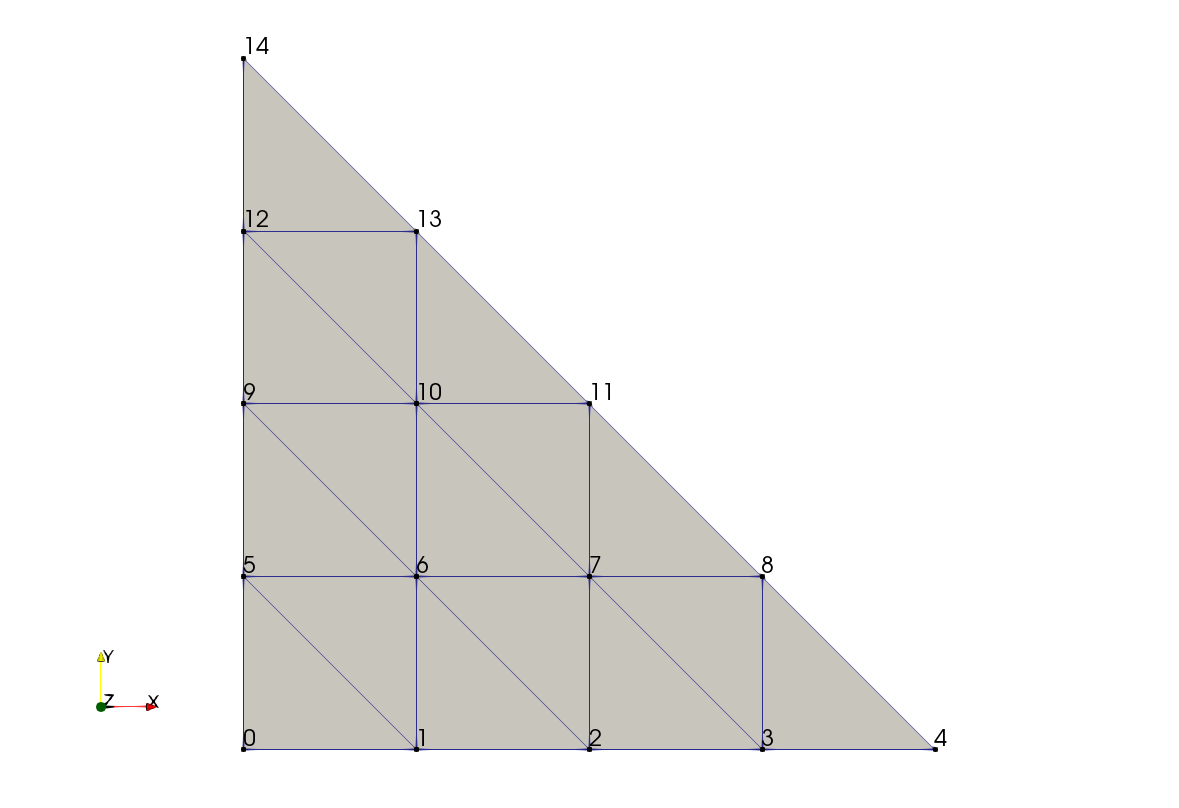
\includegraphics[width=6cm]{python_codes/fieldstone_51/minigrid5}
\end{center}




